\chapter{Schlussbetrachtung}
\label{ch:schluss}
    Das im Rahmen dieser Arbeit erarbeitete Konzept in Form eines prädiktiven Warnsystems zur Vorhersage von Filterversagen wird im folgenden bewertet. Hierbei werden die simulierten Schadenszeitpunkte mit der Vorhersage verglichen. Desweiteren wird das Potenzial einer KI-basierten Analyse aufgezeigt, indem der Warnungszeitpunkt mit dem Tauschzeitpunkt lt. Datenblatt abgeglichen wird. Es folgt eine kritische Betrachtung der vorliegenden Arbeit mit Hinblick auf die Grenzen des Konzepts und die getroffenen Vereinfachungen in der Simulation. Eine praktische Anwendung und Verfeinerung wird als Ausblick dargestellt. 
    \section{Ergebnisdarstellung}
    \label{sec:ergebnisse}
    Wie in Kap. \ref{sec:knime_auswertung} angedeutet, wurde der Workflow in \ac{KNIME} mit einer Metanode erweitert, die automatisiert folgende Ergebnisse liefert. Grund für die Automatisierung ist die Möglichkeit zur Optimierung des Modells anhand dieser praktischen Kennwerte. Als Vorhersagehorizont wurde der Zeitraum von einer Woche gewählt (s. Kap. \ref{sec:funktionsweise}). Zunächst wurde über unterschiedliche Operationen der jeweils erste Zeitpunkt des Auftretens einen vorhergesagten Schadens (First pred. Failure) mit dem ersten Auftreten eines simulierten Schadens (First real Failure) verglichen (s. Abb. \ref{fi:knime_results1}). Durch Bildung der Differenz zwischen diesen beiden Zeitpunkten wurde die dritte Zeile (delta [min]), und durch Division $\frac{min}{60}=h$ die vierte Zeile (delta [h]) berechnet. Bei der Interpretation der dargestellten Werte ist zu beachten, dass die vorgestellten Testdaten nicht zum Training des Modells genutzt wurden, und außerdem die Nutzungszeiten in der Simulation $37,5+\frac{n*10}{24} \% $ pro Tag unter Nichtbeachtung von Wochenenden betragen. Da für die Testdaten die letzten Durchläufe $n=41..50$ verwendet wurden entspricht dies einer täglichen Nutzungszeit von 
    $ 13,1...14$ Stunden. Dennoch ist der schlechteste Wert für die Vorhersage $-11,7$ Stunden, was immernoch eine Vorlaufzeit für den Tausch von $6,5$ Tagen bedeutet. Die positiven Werte bedeuten also eine frühzeitige Ausgabe der Warnung durch das Modell. Zusammenfassend lässt sich also sagen das mit dem Modell bei einer anvisierten Vorhersagezeit von einer Woche im Fall der Testdaten mindestens sechs Tage bleiben, um den Filter zu tauschen.
    \begin{figure}[h]
        \begin{center}
            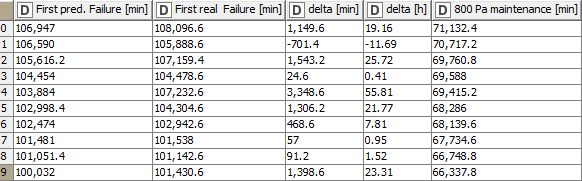
\includegraphics[width=1.1\linewidth]{images/knime_results1.png}
            \caption[KNIME Vergleich Vorhersage mit Simulationswerten]{Vergleich der Vorhersage mit simulierten Versagenszeitpunkten in KNIME}
            \label{fi:knime_results1}
        \end{center}
    \end{figure}
    
    Abb. \ref{fi:knime_results2} zeigt nun die zusätzlich erreichte Einsatzdauer des Filters, bei einem Tausch des Filters bei $\Delta p=\SI{800}{\pascal}$ in Folge einer konventionellen Filterüberwachung mit Grenzwert. Hierzu wurden die Werte der Einsatzdauern bei erster Warnung mit der Einsatzdauer bei erstmaligen Überschreiten von $\Delta p=\SI{800}{\pascal}$ verglichen (delta maintenance/pred [min]). Die zusätzlich erreichte Lebensdauer in Tagen wird in der rechten Spalte (delta maintenance/pred [d]) dargestellt. Hierbei wird also eine Verlängerung der Standzeit von $ 23,4...24,9$ Tage erreicht, was ebenfalls im Kontext der vorher erwähnten, eher ungewöhnlich langen Nutzungsperioden zu sehen ist.
    \begin{figure}[h]
        \begin{center}
            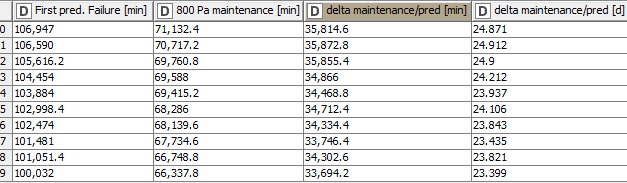
\includegraphics[width=1.1\linewidth]{images/knime_results2.png}
            \caption[KNIME Zeitgewinn durch Vorhersage]{Vergleich der Vorhersage mit Tauschzeitpunkt nach Datenblatt in KNIME}
            \label{fi:knime_results2}
        \end{center}
    \end{figure}
    \section{Kritische Würdigung}
    Ziel des KI-Modells war eigentlich eine Vorhersage der Ausfallwahrscheinlichkeit, sowie die Vorhersage unterschiedlicher Schadensarten bzw. Verschleißzustände. Dies wurde nicht erreicht. Die in Kap. \ref{sec:ergebnisse} vorgestellten Ergebnisse liefern dennoch Aufschluss über das erreichbare Potenzial einer KI-basierten Überwachung. 
    Für die Simulation war ursprünglich die Modellierung der unterschiedlichen Filtereffekte bei unterschiedlichen Umgebungsbedingungen angedacht. Die Modellierung der einzelnen Filtereffekte wurde jedoch unterlassen, da dies nach Ansicht des Verfassers, keinen Mehrwert im Sinne der Aufgabenstellung geliefert hätte. Da die Kenntniss über diese Effekte jedoch zum Verständnis der Arbeit und Filtern allgemein beitragen, sind die entsprechenden Grundlagenkapitel in der Arbeit belassen worden. Um das Simulationsmodell nicht unnötig zu verkomplizieren, und außerdem vergleichbare Reihen zu generieren wurde auf eine Simulation einer bedarfsabhängigen Regelung (IDA C5 bzw C6) verzichtet.
    Das Simulationsmodell ließe sich bei Bedarf jedoch ohne großen Aufwand dahingehend anpassen. Desweiteren wurden im Rahmen der Simulation einige Annahmen und Vereinfachungen getroffen, weswegen diese eher als Generator von Daten als eine ernsthafte Simulation zu sehen ist. Teilweise wurden fast willkürliche Anpassungen an der Simulation vorgenommen, um eine gewisse Varianz zu erreichen. Ein Beispiel hierfür wäre die Einführung von Zufall bei der Generierung der Feuchteverläufe, was zu einem verrauschten Signal geführt hat, welches schlussendlich bei der Analyse wieder geglättet werden musste.
    Die simulierten Zusammenhänge sind bei Weitem nicht vollständig. Die Temperatur wurde vollständig unterschlagen. Es lässt sich festhalten, dass der Themenkomplex Luftfilter, und deren Verhalten bei unterschiedlichen Umweltbedingungen, extrem schwierig quantifizierbar ist, was eventuell auch die relativ geringe Anzahl an Veröffentlichungen zu diesem Thema erklärt. \newline
    Allerdings vermitteln die simulierten Verläufe einen plausiblen Eindruck, und sollten daher zumindest qualitativ dem Ziel der vorliegenden Arbeit genügen.
    Dennoch deutet die angesprochene Komplexität der Zusammenhänge recht deutlich auf den Einsatz von \ac{ki}, denn die Ermittlung von Zusammenhängen und Mustern aus Datenmengen ist klassischerweise deren größte Stärke. Dies wurde durch die vorgestellten Ergebnisse aus Sicht des Verfassers auch bestätigt. Mit dem Aufkommen von codeless Software wie z.B. \ac{KNIME} zur Datenanalyse lassen sich solche Ansätze auch mit Grundlagenwissen in der Informationstechnik, sowie ausreichend Domänenwissen, realtiv schnell praktisch umsetzen. Hierfür liefert \ac{KNIME} unter anderem Schnittstellen zu Microsoft SharePoint, oder auch Möglichkeiten zum Schreiben in eine SQL-Datenbank. Eine Automatisierung der Datenanalyse, und somit z.B. Ausgabe von Warnungen in ein Wartungsplanungssystem ließe sich also schon heute realisieren. 
    \section{Ausblick}
    Die vorliegende Arbeit zielte auf die Entwicklung eines Konzepts zur KI-gestützten Messdatenauswertung von Messgrößen zur Erfassung bzw. Vorhersage von Verschleißarten.
    Die vorgestellten Ergebnisse zeigen hierbei großes Potenzial bei der Verlängerung der Standzeit, und ermöglichen außerdem eine gewisse Vorlaufzeit bei der Planung von Tauscheinsätzen zum Wechsel der Filter. Hierbei sollten jedoch der höhere Energieaufwand, der aus einer phasenweise höheren Druckdifferenz am Filter resultiert, hinsichtlich ökonomischen und ökologischen Aspekten abgewogen werden. Das vorgestellte Konzept ließe sich anhand von praktischen Versuchen und Messdaten noch weiter verfeinern. Daher sollte die Einfachheit der Simulation nicht gegen eine Sinnhaftigkeit der vorgestellten Lösung sprechen. Für eine vollständige Implementierung sind dabei vorallem die örtlichen Gegebenheiten zu berücksichtigen, so vorallem wie in Kap. \ref{ch:konzept} vorgestellt, die vorhandene \ac{glt}. Bei künftigen Untersuchungen an Filtern mit gegebenen Einsatzzeiten ließe sich mit den in Kap. \ref{sec:versuchsreihen} umrissenen Versuchsreihen das vorgestellte Modell schnell auf einen praktischen Anwendungsfall adaptieren. Schlussendlich wäre für die vollständige Integration auch die Kenntniss über vorhandene Wartungsplanungssysteme und die vorhandene IT-Infrastruktur notwendig, um eine wirtschaftlich sinnvolle Lösung zu entwickeln. Der Verfasser stellt die Anwendung des Konzepts auf einen praktischen Anwendungsfall in Aussicht. Hierbei wären die nächsten Schritte die Erlangung der fehlenden Kenntnisse, und der Aufbau eines Teststandes mit geeigneter Messtechnik zur Untersuchung der jeweiligen Filter. 